\documentclass{beamer}
\usepackage{pgfpages}
\usepackage{amsmath}
\usepackage{amsfonts}
\usepackage{fontspec}
\usepackage{xunicode}
\usepackage{xltxtra}
\usepackage{color}

\usepackage{beamertheme_atilla/beamerthemeAtilla}

\defaultfontfeatures{Mapping=tex-text}
%\setromanfont{Linux Libertine O}
\setsansfont{FreeSans}

\setbeameroption{show notes}
\setbeameroption{show notes on second screen=left}

% Hack to allow XeTeX to produce wide pdf
\renewcommand\pgfsetupphysicalpagesizes{%
	\pdfpagewidth\pgfphysicalwidth\pdfpageheight\pgfphysicalheight%
}

% CUSTOM COLORS ===============================================================

\definecolor{gray}{rgb}{0.5,0.5,0.5}
\definecolor{darkgreen}{rgb}{0.0,0.5,0.0}
\definecolor{mygreen}{rgb}{0,0.6,0}
\definecolor{mygray}{rgb}{0.5,0.5,0.5}
\definecolor{mymauve}{rgb}{0.58,0,0.82}
\definecolor{myorange}{RGB}{246,177,50}

% CUSTOM COMMANDS =============================================================

\newcommand\fixme{\textrm{\textbf{\textcolor{red}{FIXME: }}}}
\newcommand\todo{\textrm{\textbf{\textcolor{myorange}{TODO: }}}}
\newcommand\click{{\Large \textrm{\textbf{\textcolor{red}{CLICK! }}}}}
\newcommand\mytilde{\raise.17ex\hbox{$\scriptstyle\sim$}}
\newcommand\okeanos{\raise.17ex\hbox{$\scriptstyle\sim$}okeanos }
\newcommand\spc{\hfill \\}
\newcommand\dspc{\spc\spc}

\AtBeginSection[]
{
	\begin{frame}
		\frametitle{Table of Contents}
		\tableofcontents[currentsection]
	\end{frame}
}

% PRESENTATION SETTING ========================================================

\author{Αλέξιος Πυργιώτης}
\title{Σχεδίαση και Υλοποίηση Μηχανισμού Κρυφής Μνήμης για
	Κατανεμημένο Σύστημα Αποθήκευσης σε Περιβάλλον
	Υπολογιστικού Νέφους}
\institute{Εθνικό Μετσόβιο Πολυτεχνείο}
\date{\today}


\begin{document}
\chapter{Introduction}\label{ch:intro}

%In the technology race of computer components
In the new-age race of hardware, where vendors are always trying to produce the 
next record-breaking unit, be it CPU, RAM or network cards, hard disks seem old 
and gasping to catch up. For decades now, their sub-par performance, compared 
to volatile memory, has been the bottleneck of every IO-intensive application 
and the headache of storage designers \cite{nvm}. As over-stretched as this may 
seem, it is a fact that it has shaped the way storage is built; from the common 
computer (Linux's page cache, Bcache) to large deployments (the memcached 
servers of Facebook and Twitter \fixme add paper), there is a tremendous effort 
from the research and corporate community that is being invested in 
sidestepping hard disks and finding alternative methods to store data.

The hard disks' industry answer to this is the continuous drop of their prices.  
In 2011 (\fixme be more specific), the HDDs reached their all-time low price of 
\$0.053/GB \cite{hdd-price}. Moreover, the emerging movement of greener data 
centers has benefited hard disks, since their low energy costs has been proved 
attractive to the enterprises. Yet, for how long can the HDD industry keep 
lowering the costs to mitigate their lack of performance?

The answer came very fast and unfortunately in a tragic way. The end of July of 
2011 marked the beginning of a 6-month turmoil for Thailand, with a flood that 
was described as "the worst flooding yet in terms of the amount of water and 
people affected" \cite{flood}. The hard disk industry also suffered a huge hit 
due to the fact that 25\% percent of the global hard disk production was from 
factories in Thailand, that were also affected by the flood.

The result was an overnight 40\% percent increase of hard disk prices. The 
reasons behind this increase were partly to compensate for the flood damages 
and partly to seize the opportunity to increase the profit margins of the two 
biggest producers, Western Digital and Seagate, from 6\% and 3\% to 16\% and 
37\% respectively \cite{rosenthal12-unesco}.

The timing could not have been worse for the HDD industry. This increase in 
price introduced SSDs who are now starting to be considered as a viable 
solution for peripheral storage tasks such as journaling and caching, due to 
their high performance and their persistence, which separates them from other 
volatile storage types.

On the other hand, the current situation is that HDDs can only marginally 
improve their performance. As their rotational speed approaches the speed of 
sound, their production will be rendered at best difficult, and their heat 
generation, power consumption and lack of long-term reliability will make their
adoption prohibitive \cite{hddtrends},\cite{speed-of-sound}.

The cloud world is largely affected by the future of storage mediums. Besides 
SSDs, there are various other non-volatile storage types that are trying to 
race for the momentum




\todo Explain in a few words what we are trying to do here and why.


\section{Thesis structure}

\fixme Fix the summary and references of these chapters.

% TODO: Make Chapter x click-able and anchored to the respective chapter

\begin{description}
\item[Chapter~\ref{ch:ch2}:]
We define what "cloud" means and mention some of the most notable examples.
Then, we give a brief overview of the synnefo implementation, its key
characteristics and why it can have a place in the current cloud world.
\item[Chapter~\ref{ch:archipelago}:]
We present the architecture of Archipelago and provide the necessary 
theoretical background (mmap, IPC) the reader needs to understand its basic 
concepts. Then, we thoroughly explain how Archipelago handles I/O requests.  
Finally, we mention what are the current storage mechanisms for Archipelago and 
evaluate their performance.
\item[Chapter~\ref{ch:tiering}:]
We explain why tiering is important and what is the state of tiered storage at
the moment (bcache, flashcache, memcached, ramcloud, couchbase).  Then, we
provide the related theoretical background for cached (hash-tables, LRUs).
Finally, we defend why we chose to roll out our own implementation.
\item[Chapter~\ref{ch:cached-design}:]
We explain the design of cached, the building blocks that is consisted of
(xcache, xworkq, xwaitq). Then, we give some examples that illustrate the 
operation under different scenarios
\item[Chapter~\ref{ch:cached-implementation}:]
We present the cached implementation, the structures that have been created and 
the functions that have been used.
\item[Chapter~\ref{ch:cached-evaluation}:]
We explain how cached was evaluated and present benchmark results.
\item[Chapter~\ref{ch:synapsed}:]
It connects brain parts. And its tale must be told.
\item[Chapter~\ref{ch:ch7}:]
We draw some concluding remarks and propose some future work.
\end{description}

\section{VM Volume storage}

\begin{frame}[t]{Intro}

	\note[item]{Σε μεγάλες εγκαταστάσεις, ξεφεύγουμε από το κλασσικό 
		μοντέλο του PC μας (το μηχάνημα έχει το σκληρό του δίσκο).  
		Συγκεκριμένα σε μια cloud υποδομή έχουμε:}
	\note[item]{\click}
	\note[item]{To VM που τρέχει σε ένα host server}
	\note[item]{\click}
	\note[item]{Και τους storage servers}
	\note[item]{\click}
	\note[item]{Το ερώτημα είναι λοιπόν, πως το VM θα αποθηκεύει τα 
		δεδομένα του;\\
		Υπάρχουν διάφορες επιλογές όπως το DRBD, το RBD που 
		χρησιμοποιούνται ευρέως και γεφυρώνουν τον αποθηκευτικό χώρο 
		του VM με το χώρο όπου λειτουργεί.}
	\note[item]{Τι γίνεται όμως στην περίπτωση που θέλουμε *και* τα εξής;}
	\note[item]{\click}
	\note[item]{Εξήγησε τους όρους}

	\begin{columns}[t]
		\begin{column}{.5\textwidth}
			\pause
			\makebox[\textwidth]{\includegraphics[width=.2\paperwidth]{images/vm.jpg}}
			\pause \centering{ {\Huge +} }
				\makebox[\textwidth]{\includegraphics[width=.2\paperwidth]{images/cloud-server1.jpg}}
			\pause \centering{ {\Huge = ?}}
		\end{column}
		\begin{column}{.5\textwidth}
			\pause
			\begin{itemize}
				\item Policy enforcement?
				\item Storage agnosticity?
			\end{itemize}
		\end{column}
	\end{columns}

\end{frame}

\begin{frame}{Our solution}

	{\Large Archipelago}

	\makebox[\textwidth]{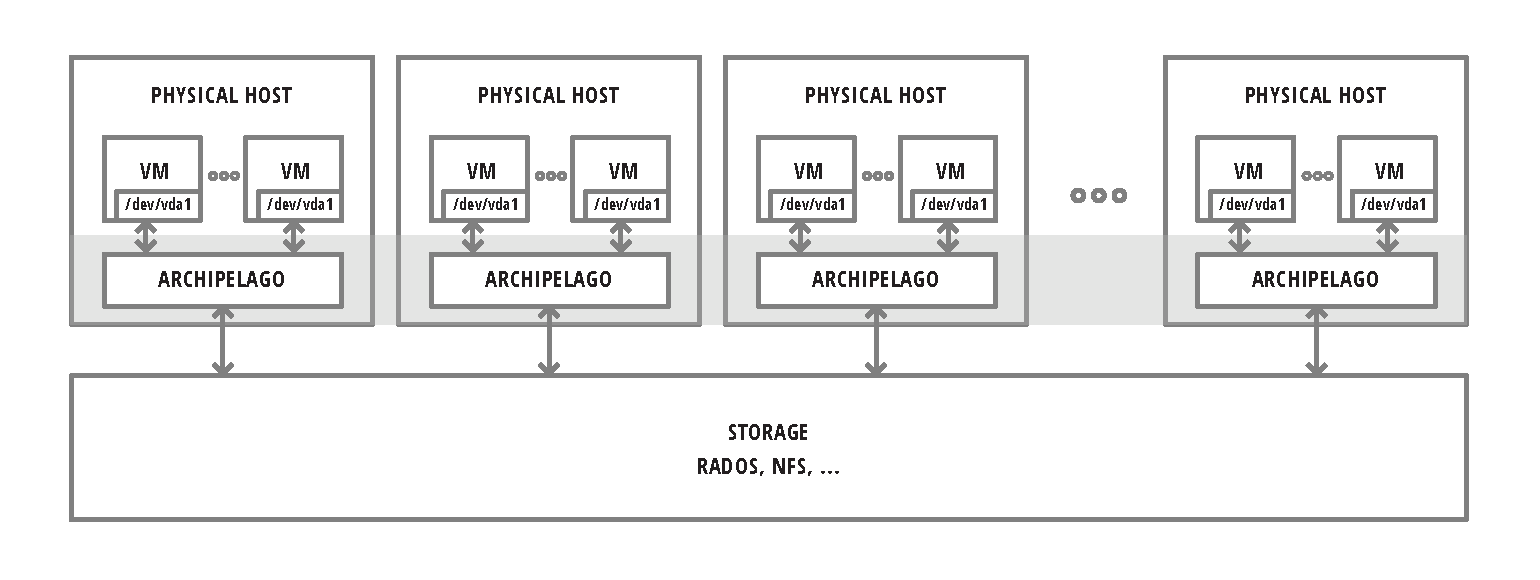
\includegraphics[width=\textwidth]{images/archipelago_overview_a.pdf}}

	\spc

	Key features:
		1) Software-defined
		2) Distributed
		3) Modular
		4) Copy-On-Write
		5) Storage agnostic

	\note{Η λύση που χρησιμοποιήσαμε είναι το Archipelago}
	\note{
		\begin{itemize}
			\item Software-defined: αν και είναι ένα όρος 
				μαρκετινγκ, εμείς κανονικά. Σημαίνει με το 
				software ΟΡΙΖΕΙΣ το storage (εφαρμογή policy, 
				αλλαγή πορείας του request)
			\item τρέχει σε πολλούς κόμβους
			\item αποτελείται από διακριτά κομμάτια
			\item κάνει CoW (εξήγησε ότι τα images είναι λίγα, τα
				VMs πολλά, όπως όταν ένα process κάνει fork)
			\item μπορούμε χρησιμοποιήσουμε ότι storage θέλουμε
		\end{itemize}
	}

\end{frame}

\begin{frame}{Archipelago Architecture}
	%\includegraphics[{images/new_sxima_numbered.pdf}
	\begin{center}
		  \makebox[\textwidth]{\includegraphics[width=0.9\paperwidth]{images/new_sxima_numbered.pdf}}
	\end{center}

	\note[item]{To VM στέλνει αίτημα στο δίσκο του, ο δίσκος είναι εικονικός, 
		θα το δει ο hypervisor (εξήγησε τι είναι ο hypervisor) και θα το 
		στείλει στον δίσκο που το έχουμε πει. (xsegbd)}
	\note[item]{Ο xsegbd στέλνει τo αίτημα στο userspace κομμάτι του 
		Αρχιπελάγους το οποίο αποφαίνεται για τα αντικείμενα τα οποία 
		αντιστοιχούν στο αίτημα. Συνοπτικά πως γίνεται αυτό:
		\begin{itemize}
			\item Ο xsegbd στέλνει το αίτημα στο vmlmc
			\item Ο vlmc συμβουλεύεται τα mappings του
		\end{itemize}
	}
	\note[item]{μετά τα ζητάει από το storage μέσω των blockers}
\end{frame}

\begin{frame}{RADOS}

	The object store component of Ceph filesystem.\\
	\spc
	Key features:
	\begin{itemize}
		\item Replication
		\item Fault tolerance
		\item Self-management
		\item Scalability
	\end{itemize}

	\note{Αν και είμαστε storage agnostic, χρησιμοποιούμε ένα σημαντικό 
		storage backend, το RADOS, που μας δίνει τα εξής:
		\begin{itemize}
			\item Αντίγραφα ασφαλείας των δεδομένων
			\item Ανοχή στο χάσιμο αποθηκευτικών κόμβων
			\item Load balancing και αυτοδιαχείριση
			\item και τέλος ειναι επεκτάσιμο
		\end{itemize}
		\spc\click
	}

	\pause

	\spc
	Speed issues:\\
	VM with page-cache: > 90MB/s, < 1ms\\
	VM without page-cache: < 7MB/s, \mytilde10ms

	\note{Αυτό το περίπλοκο σύστημα όμως δεν είναι αρκετά ταχύ.  
		Παράδειγμα...
		\spc\click}
	\pause

	\spc
	Thesis goal: make this faster.

\end{frame}


\section{Caching}

\begin{frame}{Intro}

	Solution: Caching\\
	\spc
	Caching is:
	\begin{itemize}
		\item We have a slow medium
		\item Add a fast medium in a data path
		\item Transparently store the data that are intended for the 
			slower medium.
		\item Profit: later accesses to the same data are faster
	\end{itemize}
	\dspc
	Sounds familiar?

	\note[item]{Η κλασσική λύση σε τέτοια προβλήματα είναι η χρήση ενός 
		γρηγορότερου αποθηκευτικού μέσου για caching.}
	\note[item]{Για όσους δεν ξέρουν τι σημαίνει caching, θα το εξηγήσουμε 
		συνοπτικά: έχεις ροή, αργό μέσο, βάζεις ένα γρήγορο, speedup}
	\note[item]{Προφανώς αυτό το concept είναι γνωστό. Από που;}
\end{frame}

\begin{frame}
	\makebox[\textwidth]{\includegraphics[width=0.8\textwidth]{images/mem-hier.pdf}}
	
	That's because every PC is built that way.

	\note[item]{Από το ιεραρχικό μοντέλο του υπολογιστή: cpu cache vs ram, ram 
		vs disk}
\end{frame}

\begin{frame}
	Is there anything to help us?
	\dspc
	FACT: We are not the first to have speed issues\\
	Facebook, Twitter, Dropbox, every one has hit and surpassed their limits.
	\dspc
	There are solutions separated in two categories:
	\begin{itemize}
		\item Block-based caching
		\item Object-based caching
	\end{itemize}
	\note[item]{Τώρα που ξέρουμε τη λύση, υπάρχει κάτι που μπορούμε να 
		κάνουμε;}
	\note[item]{Υπάρχει κάτι έτοιμο; ΝΑΙ}
	\note[item]{Δυο κατηγορίες:
		\begin{itemize}
			\item βλέπουν τα δεδομένα σαν blocks ενός δίσκου
			\item βλέπουν τα δεδομένα σαν κομμάτια αντικειμένων
		\end{itemize}
		Διαφορά: \todo
	}
\end{frame}

\begin{frame}{Block-based caching solutions}

	Most notable examples:
	\begin{itemize}
		\item Bcache
		\item Flashcache
		\item EnhanceIO
	\end{itemize}
	\dspc
	Typically scale-up solutions.
	\dspc
	Pros: Simple, scale-up\\
	Cons: Unaware of CoW, kernel solutions

	\note[item]{Δε θα επεκταθούμε γιατί έχουν κάποια βασικά κοινά:
		\begin{itemize}
			\item Kernel modules
			\item expose εικονικά block devices που δείχνουν σε 
				γρήγορα μέσα
			\item Καθαρά caching μηχανισμοί με policies
		\end{itemize}
	}
	\note[item]{Εξήγησε που μπαίνουν (xsegbd). ΠΗΓΑΙΝΕ στο archipelago}
	\note[item]{Παρότι είναι αρκετά απλοί, δε γνωρίζουν την CoW πολιτική 
		άρα χάνουν χώρο και είναι στον kernel (που δε θέλουμε)
	}
\end{frame}

\begin{frame}{Object-based caching solutions}
	Most notable examples:
	\begin{itemize}
		\item Memcached
		\item Couchbase
	\end{itemize}
	\dspc
	Typically scale-out solutions
	\dspc
	Pros: Distributed with no SPOF, can utilize unneeded RAM\\
	Cons: Memcached has no persistence, Couchbase cannot use RADOS as its 
	backend, more suitable for databases
	\note{Τα πράγματα γίνονται πιο ενδιαφέροντα εδώ:
		\begin{itemize}
			\item Κατανεμημένα συστήμα χωρίς ενιαίο σημείο 
				αποτυχίας (SPOF), μπορούν να τρέχουν εκτός host 
				οπότε δεν το επιβαρύνουν
			\item Memcached δε διατηρεί τα δεδομένα, couchbase δεν 
				μπορεί να μιλήσει με rados
		\end{itemize}
	}
\end{frame}

\begin{frame}{Page-cache?}

	What if we used the page-cache?
	\note{Αν χρησιμοποιούσαμε την page-cache}
	\dspc
	\dspc
	\dspc
	Pros: Easy to activate, tested, very fast\\
	Cons: Unaware of CoW, no control over it, practically kernel solution\\
	\note{Εύκολη λύση, σταθερή και γρήγορη. Όμως, δεν καταλαβαίνει από COW, 
		είναι προσκολλημένη σε ένα block device}

\end{frame}

\begin{frame}{Conclusions}

	\begin{itemize}
		\item Most solutions far from Archipelago's logic
		\item Others not suited for storage and more suited for 
			databases
		\item Block-based caching might be good for the storage backend
		\item Must implement our own solution
	\end{itemize}

	\note{\todo}
\end{frame}
	

\section{Cached design}

\begin{frame}{Requirements}

	Design goals for cached:
	\begin{itemize}
		\item Create something close to the Archipelago logic
		\item Measure the best possible performance we can get
	\end{itemize}

	\note{Επιλέξαμε λοιπόν να δημιουργήσαμε τη δική μας λύση. Την ονομάσαμε 
		cached από το cache daemon}
	\note{Ορίσαμε τους εξής γενικούς στόχους:
		\begin{itemize}
			\item Να είναι κοντά στη λογική του Archipelago
			\item Η υλοποίηση να είναι όσο το δυνατόν πιο γρήγορη 
				για να δουμε αν μια Αρχιπελαγική λύση μας 
				βοηθάει
		\end{itemize}
	}
	\dspc
	Stricter requirements for cached:
	\begin{itemize}
		\item Nativity
		\item Pluggability
		\item In-memory
		\item Low indexing overhead
	\end{itemize}
	\note{Ακόμα, θέσαμε κάποιες πιο αυστηρές απαιτήσεις για την υλοποίηση 
		μας: 1)να είναι peer του Archipelago, 2) να μπορεί να ενεργοποιείται 
		και να απενεργοποιείται σε ένα σύστημα που είναι εν λειτουργία, 3)να 
		χρησιμοποιεί τη RAM, 4)ο indexing μηχανισμός να είναι γρήγορος}
\end{frame}

\begin{frame}{Cached design}
	\note{Εδώ βλέπουμε το design του cached. Ο cached μπαίνει ανάμεσα στον vlmc 
		και στον blocker και cach-άρει ότι άιτημα για αντικείμενα πάει στο 
		storage}
	\note{Οι εργασίες του cached χωρίζονται σε 5 κατηγορίες:}
	\note[item]{Στην διαχείριση των αιτημάτων από και προς vlmc, blocker}
	\note[item]{Στο indexing (εύρεση και καταχώρηση) των αντικειμένων}
	\note[item]{Στην υπο συνθήκες εκτέλεση εργασιών}
	\note[item]{Στην ασφαλή μετάδοση των cachαρισμένων δεδομένων στο 
		storage}
	\note[item]{Καθώς επίσης και στην ασφαλή επεξεργασία των cachαρισμένων 
		δεδομένων}
	\note[item]{\click}

	\begin{columns}[T]
		\begin{column}{0.65\textwidth}
			\includegraphics<1>[width=\columnwidth]{images/cached-design2.pdf}
			\includegraphics<2>[width=\columnwidth]{images/cached-design-comp2.pdf}
		\end{column}
		\begin{column}{0.35\textwidth}
			\includegraphics[width=\columnwidth]{images/new_sxima_numbered.pdf}
		\end{column}
	\end{columns}
	\note[item]{Και εδώ βλέπουμε τα διακριτά κομμάτια κώδικα που υλοιποιούν τα 
		παραπάνω και τα οποία θα συζητήσουμε ευθύς αμέσως}
\end{frame}

\begin{frame}{Xcache design}
	\centering\includegraphics<1>[height=0.6\textheight]{images/xcache-design.pdf}
	\centering\includegraphics<2>[width=\textwidth]{images/xcache-entry.pdf}

	Xcache is responsible for: 1) entry indexing, 2) entry eviction, 3) 
	concurrency control

	\note[item]{Αυτό είναι το xcache, που είναι υπεύθυνο για την
		\begin{itemize}
			\item Indexing των αντικειμένων
			\item Eviction αντικειμένων από την cache με τη χρήση LRU
			\item Χειρισμό πολλαπλών threads
		\end{itemize}
	}
	\note[item]{Έχουμε δυο hash table, το καθένα με το δικό του lock, ένα χώρο 
		που αποθηκεύονται τα entries και μόνο (όχι τα δεδομένα, προσοχή) και 
		μια στοίβα όπου κρατιούνται indexes των ελεύθερων entries.}
	\note[item]{To ένα hash table <αυτό> που κρατάει τα ονόματα των cached 
		αντικειμένων.}
	\note[item]{Ο αποθηκευτικός τους χώρος είναι preallocated και είναι <αυτό>.  
		Σε αυτό το χώρο, η αναφορά γίνεται με δείκτες. Ο ελεύθερος χώρος είναι 
		στη στοιβα αυτή.  Τέλος, όταν ένα αντικείμενο φύγει, μένει σε αυτό το 
		hash table μεχρι να το ξαναζητήσουν ή να το διωχτεί}
	\note[item]{\click}
	\note[item]{Κάθε item έχει ένα reference counter για να ξέρουμε πόσοι 
		το χρησιμοποιούν, όνομα, lru}
	\end{frame}

\begin{frame}{Xworkq design}
	\centering\includegraphics<1>[width=\textwidth]{images/xworkq-design.pdf}

	Xworkq is responsible for concurrency control
	\note[item]{xworkq υπεύθυνο για την ασφαλή επεξεργασία των δεδομένων 
		ενός αντικείμενου.}
	\note[item]{Το spinning είναι αργό, όλοι τοποθετούν μια δουλειά, ένας 
		την εκτελεί.}
	\end{frame}

\begin{frame}{Xwaitq design}
	\centering\includegraphics<1>[width=\textwidth]{images/xwaitq-design.pdf}

	Xwaitq is responsible for deferred execution
	\note[item]{xwaitq υπεύθυνο για την κατά συνθήκη εκτελεση εργασιών}
	\note[item]{Αν π.χ. μας τελειώσει ο χώρος, δεν μπορούμε να περιμένουμε 
		σύγχρονα. To thread μπορεί να τοποθετήσει μια δουλειά και μετά 
		να εκτελέσει κάτι άλλο}
\end{frame}

\begin{frame}{Bucket pool}
	When an object is indexed, it does not have immediate access to 4MB 
	size of data because:
	\begin{itemize}
		\item RAM is limited
		\item Leads to small number of entries
	\end{itemize}
	\note[item]{Το ότι κάνουμε index ένα object δε σημαίνει ότι κατ'ευθείαν 
		μπορούμε να γράψουμε σε αυτό}
	\note[item]{Δεν υπάρχει τόση RAM και ακόμα και ως αποτέλεσμα, θα 
		cachάραμε μικρό αριθμό από objects}
	Ideally, we want to:
	\begin{itemize}
		\item Decouple the objects from their data
		\item Cache unlimited objects but put a limit on their data
	\end{itemize}
	\note[item]{Ιδανικά θέλουμε να διαχωρίσουμε την καταχώρη/όνομα του 
		αντικειμένου από τα δεδομένα του. Δυνητικά θα μπορούμε να 
		καταχωρούμε πάρα πολλά αντικείμενα αλλά θα έχουμε μικρότερο 
		χώρο}

	Solution:
	\begin{itemize}
		\item Preallocated data space
		\item Every object request a bucket (typically 4KB)		
		\item When an object is evicted, its buckets are 
			reclaimed
	\end{itemize}
	\note[item]{Preallocated χώρος, όλοι παίρνουν indexes από αυτό (Θυμίζει 
		xcache}
\end{frame}

\begin{frame}{Other important cached tasks}

	Several other key-tasks are:
	\begin{itemize}
		\item Book-keeping
		\item Cache write policy
		\item Asynchronous task execution
		\item Data propagation
	\end{itemize}
	\note{Το cached είναι επίσης επιφορτισμένο και με άλλες δουλειές όπως:
		\begin{itemize}
			\item Κρατάει στατιστικά (πόσα entries είναι dirty, 
				πόσα buckets έχει κάνει allocate ένα entry
			\item Εφαρμόζει writeback/writethrough πολιτική
			\item Φρόντίζει ώστε οι εργασίες να μπορούν να γίνουν 
				ασύγχρονα
			\item Και φυσικά φροντίζει τα δεδομένα να γράφονται 
				σωστά στο storage
		\end{itemize}
	}
\end{frame}

\begin{frame}{Cached flow}
	\includegraphics<1>[height=0.8\textheight]{images/cached-design2.pdf}
	\includegraphics<2>[height=0.8\textheight]{images/cached-design-comp2.pdf}

	\note[item]{Εδώ παίζεις με τα slides}
	\note[item]{Θα παρουσιάσουμε πολύ γρήγορα τη ροή ενός αιτήματος στον 
		cached}
	\note[item]{Έρχεται request, το κάνουμε index, μπαίνουμε στη workq και 
		πειράζουμε τα δεδομένα του και ανάλογα το cache policy το 
		γράφουμε πίσω στον blocker αλλιώς τελειώσαμε}
	\note[item]{Optional σεναρια:
		\begin{itemize}
			\item Αν γίνει ένα eviction, πρέπει να γράψουμε τα 
				δεδομένα του πίσω με ασφάλεια. Επειδή το 
				αντικείμενο μπορει να καταχωρηθεί, να μπει και 
				να ξαναβγεί, πρέπει να είμαστε προσεκτικοί
			\item Αν ξεμείνουμε από πόρους (χώρο στο hash table, 
				buckets κτλ, πρέπει να συνεχίσουμε μονο όταν 
				μπορούμε
		\end{itemize}
	}
\end{frame}

\chapter{Performance evaluation of cached}\label{ch:cached-evaluation}

\begin{flushright}
	\textit{"There are three kinds of lies:\\
		lies, damned lies, \\
		and \sout{statistics} benchmarks."}	\\

	Mark Twain (modernized)
\end{flushright}

It may seem as an ironic statement, considering that we are about to provide 
benchmark results for cached, but it's actually is a valid one.
\begin{comment}
What Mr.  Twain tries to say here
\footnote{
	and that's a phrase usually not heard in programming contexts...
}
is that the presentation of partials facts for something can be used to 
fabricate a plausible truth for it.
%This is shit, fix it
In science's case, it so often happens that promising results for an experiment 
can seem more important to the researcher's eye than negative ones due to 
positive reinforcement.
\end{comment}
In our case, we will try not to merely smear the next pages with diagrams but 
first explain the benchmarking methodology behind them and then provide a 
concrete depiction of cached's performance under various workloads.

The skeleton of this chapter is the following: Section \ref{sec:perf-meth} 
explains the methodology behind our measurements. Section \ref{sec:test-bed} 
provides details about the hardware on which we have conducted our benchmarks.  
Section \ref{sec:perf-plot} presents the results of the benchmarks that we have 
conducted and provides in-depth explanations about each of them.  Finally, 
Section ?  is reserved for cached on a VM (\fixme take these measurements).

\section{Benchmark methodology}\label{sec:perf-meth}

The benchmarks that have been executed and whose results are presented in this 
chapter, will be split in two categories, both of which have their own distinct 
goals:

The first category is the comparison between using cached \textbf{on top} of 
the sosd peer (sosd has been discussed here ? \fixme add section) and using 
solely the sosd peer.

\begin{comment}
The category's goal is to "defend" one of the core thesis arguments, that 
tiering is a key element that will improve the performance of Archipelago.  
\end{comment}

In order to effectively compare the performance of cached and sosd, we must 
consider the following: 

\begin{enumerate}
	\item The comparison of the two peers should try to focus on what is 
		the best performance that these peers can achieve for a series 
		of tough workloads.
	\item The circumstances under which both peers will be tested need not 
		be thorough but challenging. For example, it may be interesting 
		to test both peers against sequential requests, but
		\begin{inparaenum}[i)]
		\item such patterns are rarely a nuisance for production 
			environments
		\item they do not stress the peers enough to provide something 
			conclusive
		\item they are out of the scope of this section as there can be 
			many of these kinds of tests and adding them all here 
			will impede the document's readability.
		\end{inparaenum}
	\item Both peers must be tested under the same, reasonable workload, i.e a 
		workload that can be encountered in production environments.
	\item If the peer doesn't show a consistent behavior for a workload, it 
		must be depicted in the results.
\end{enumerate}

Having the above in mind, the next step is to choose a suitable workload.  This 
choice though is fairly straight-forward; in production environments, the most 
troublesome workload is the burst of small random reads/writes and is usually 
the most common one that is benchmarked.  

One may ponder however, how many requests can be considered as a "burst" or 
which block size is considered as "small". Of course, there is not only one 
answer to this question so, we will work with ranges. For our workload, we will 
use block sizes ranging from 4KB to 64KB and parallel requests ranging from 4 
to 16.

The second category deals solely with the inner-workings of cached and its 
behavior on different operation modes or states. Its aim is not to capture the 
performance against a tough workload, but to explain \textbf{why} this 
performance is observed and how each of the options affect it. In this 
category, we measure how threads impact the performance of cached or what 
impact (if any) does our index mechanism have.

Finally, in the following sections, for brevity reasons, we will talk about 
comparing cached and sosd. What the reader must keep in mind however is that 
cached is essentially the cache layer above sosd, which means that we actually 
test sosd vs cached over sosd.

\section{Specifications of test-bed}\label{sec:test-bed}

The specifications of the server on which we conducted our benchmarks is the 
following.

\begin{table}[H]
	\centering
	\begin{tabular}{ | l | l | }
		\hline
		Component & Description \\ \hline \hline
		CPU &  2 x Intel(R) Xeon(R) CPU E5645 @ 2.40GHz \cite{e5645} \\
		 & Each CPU has six cores with Hyper-Threading enabled, which equals to 
		 24 threads. \\ \hline
		RAΜ & 2 banks x 6 DIMMs PC3-10600 \\
		& Peak transfer rate: 10660 MB/s \\ \hline
	\end{tabular}
	\caption{Test-bed hardware specs}
	\label{tab:hardware-specs}
\end{table}

\begin{table}[H]
	\centering
	\begin{tabular}{ | l | l | }
		\hline
		Software & Version \\ \hline \hline
		OS &  Debian Squeeze \\ \hline
		Linux kernel & 3.2.0-0 (backported) \\ \hline
		GCC & Debian 4.4.5-8 \\ \hline
	\end{tabular}
	\caption{Test-bed software specs}
	\label{tab:software-specs}
\end{table}

\todo add configuration of RADOS cluster (journal, backing storage, network 
connection)

\fixme Mention that the peers were evaluated by sending requests directly at 
their ports.

\section{Performance comparison between cached and sosd}
\label{sec:perf-plot}

As mentioned above, for our first test, we will evaluate the read and write 
performance of cached and sosd for a random workload with parallel requests of 
small size. In order to measure accurately their performance, we will use two 
different metrics:

\begin{description}
	\item[Bandwidth:] \hfill \\
		Bandwidth measures the maximum throughput that the application 
		can sustain. This metric is usually used to indicate how much 
		I/O (from various inputs) can an application handle within a 
		second.
	\item[Latency:] \hfill \\
		Latency is the converse of bandwidth. It is a measurement from 
		the viewpoint of the issuer of requests and indicates the 
		responsiveness of the tested application. It is commonly 
		calculated as the average reply time for a series of requests.
\end{description}

On the following sections, we present the benchmarks that we conducted for the 
first category. The first benchmark, which is shown in Section 
\ref{sec:peak-plot} attempts to depict the behavior of cached during a peak of 
I/O requests. The second benchmark, which is shown in Section 
\ref{sec:sustained-plot}, illustrates the behavior of cached under continuous 
load.  On these sections, cached is always multi-threaded and uses 4 threads.

\subsection{Workload smaller than cache size - Peak behavior}
\label{sec:peak-plot}

We begin with the bandwidth performance of our peers. The write performance can 
be seen in Figure \ref{fig:bw-write-comp-lie.pdf} while the read performance 
can be seen in Figure \ref{fig:bw-read-comp-lie.pdf}.

Before we proceed with the interpretation of the diagram results, we will 
briefly comment on the diagram structure. Due to the fact that the performance 
of the two peers differs in at least two orders of magnitude, the results would 
look too flat in a conventional diagram that would scale from 0 to 11000. To 
amend this, we have broken the y-axis of our diagrams in two parts with 
different scales and starting values, in order to make the comparison easier to 
the eye.

\diagram{Comparison of bandwidth performance for write 
	peaks}{bw-write-comp-lie.pdf}
\diagram{Comparison of bandwidth performance for read 
	peaks}{bw-read-comp-lie.pdf}

The initial results look very promising. For write requests, the speedup for 
very small block sizes (4KB - 16KB) is approximately \textbf{100x} whereas for 
larger ones (32KB - 64KB) it ranges from \textbf{50x to 200x}. For read 
requests, the speedup for very small block sizes is approximately \textbf{50x}, 
whereas for larger block sizes, it ranges between \textbf{20x - 75x}.

These results not only illustrate the performance gap between RAM and
HDDs but also show that our implementation manages to keep its bandwidth 
consistently over 1 GB/s in stress scenarios. However, we must keep in mind 
that they only show a part of the full picture, since it does not show how 
cached behaves past its cache size.

Moreover, upon closer inspection the following questions arise:

\textbf{1) Where is the speedup difference between reads and writes attributed 
	to?}

We have mentioned above that the speedup for writes is between 50x and 200x 
whereas for reads is between 20x and 75x. Although it is a large speedup in 
both cases, it also shows some of the shortcomings of our implementation.

We attribute the speedup difference to three factors:

\begin{enumerate}
	\item The performance of cached is almost the same for writes and 
		reads.  This is expected behavior as the read and write paths 
		for cached have many common parts (\fixme show write/read path)
		\footnote{To be more strict, reading seems a bit faster than 
			writing, but that is probably attributed to CPU caches 
			and the fact that reading from RAM is a non-destructive 
			operation in contrast to writing.}.
	\item Cached doesn't scale much past the 16KB block size. This is an 
		interesting observation with an unexpected answer. It may seem 
		implausible at first, but what happens is that we are actually 
		hitting the bandwidth limit of the RAM modules. If we consult 
		the table \ref{tab:hardware-specs}, we can see that the 
		bandwidth limit of the RAM is about \mytilde10.7GB/s
		\footnote{A more careful look shows that we surpass this limit, 
			which is expected given the fact that we have a multi 
			channel RAM setup.}.
		This limit is approached asymptotically as the block size 
		increases and the index overhead decreases (more about the 
		index overhead later in the measurements of Section ? \fixme 
		add section).
	\item On reads, sosd is benefited from the existence of caches in 
		various levels e.g. on OSD level, on RAID controller level.
\end{enumerate}

To sum up, the cached's performance remains relatively the same in both reads 
and writes, it is merely the sosd that is getting faster in reads due to 
caches. 

\textbf{2) Why is cached's performance increased along with block size?}

We expected that sosd's performance would increase proportionally to the block 
size, due to the rotational nature of hard disk drives, but why does this 
affects cached too? It is certainly not attributed to any \texttt{memcpy()} 
performance tricks, since we always write in bucket granularity, which means 
that a 16KB write is translated to 4 x 4KB writes.

From this observation, we extrapolate that the CPU operations such as indexing,
job enqueuing, accepting and responding requests, that occur proportionally 
more times for smaller block sizes, dominate the cached's performance.

We can see this more clearly if we consult Table \ref{tab:2threads}.

\begin{table}[H]
	\centering
	\begin{tabular}{ | l | l | l | l | l |}
		\hline
		Bandwidth (MB/s) & IOPS	  & Latency (usec) & Iodepth& Block size (KB) \\ \hline \hline
  2652.327   &	678995.620& 5.002&	4&		4 \\ \hline
  4427.89l   &	566769.888& 6.176&	4&		8 \\ \hline
  5900.719   &	377646.042& 9.672&	4&		16 \\ \hline
  6895.167   &	220645.338& 17.179&	4&		32 \\ \hline
  7090.661   &	113450.584& 34.237&	4&		64 \\ \hline

	\end{tabular}
	\caption{Write performance results for 2-threaded cached}
	\label{tab:2threads}
\end{table}

\fixme elaborate on that

Merely using two threads instead of four lessens the performance gap 
significantly.

\textbf{3) Why cached's perforance does not improve proportionally to the 
	parallel requests?}

The reason why we see only a minor increase in the performance of cached, even 
though it is multi-threaded, is because our locking scheme is not fine-grained 
enough. We have a single lock for our request queue, a single lock for most of 
the hash table accesses and this inevitably causes a lot of threads to spin.  
This slight improvement we see is mainly due to the fact that requests are 
effectively being pipelined while waiting each other to release its lock.  

We now proceed to the latency results. The write performance can be seen in 
Figure \ref{fig:lat-write-comp-lie.pdf} while the read performance can be seen 
in Figure \ref{fig:lat-read-comp-lie.pdf}.

\diagram{Comparison of latency performance for write 
	peaks}{lat-write-comp-lie.pdf}
\diagram{Comparison of latency performance for read 
	peaks}{lat-read-comp-lie.pdf}

The latency results corroborate the observations that we made for the bandwidth 
results. As we can see, the latency of cached is proportional to the number of 
parallel requests, which reinforces the assumption that our locking scheme is 
not granular enough, whereas sosd has only a small variance.

\subsection{Workload larger than cache size - Sustained behavior}
\label{sec:sustained-plot}

We now proceed to the second part of the comparison between cached and sosd.  
On this part, we will once again evaluate their performance against a random 
workload with many parallel requests. Unlike the first part though, where the 
cache size was larger than the workload, on this part the cache size will
only be half of it. Having a smaller cache than the workload is after all the 
most common scenario for production environments and the results should 
complete the picture of cached's behavior in a production environment.

For this test, there are two main parameters we must take into account: the 
cache size and the maximum objects. These parameters have been decoupled in our 
implementation and we expect different results for each combination. More 
specifically, we have tested cached with half the workload size and:

\begin{enumerate}
	\item half the objects of the workload (referenced as 
		\textbf{cached-limited} from now on).
	\item more than the objects of the workload (referenced as 
		\textbf{cached-unlimited} from now on).
\end{enumerate}

Also, we have tested cached in write-through mode, to see its behavior in 
sustained writes. \fixme say it has unlimited objects 

Furthermore, for this benchmark, we tested only the write performance of cached 
and sosd.  Also, we chose to use 16 parallel requests and 4KB block sizes, 
since these seemed the most troublesome in the previous benchmark.

Before we proceed to the results, we must explain first how the diagrams below 
are structured. Since cached's performance is fairly unstable in this scenario, 
we have chosen to illustrate it as the benchmark progresses.  Thus, the x-axis 
shows what percent of the benchmark has been completed and for every 5\%, we 
show the performance of cached for that part.

The bandwidth results can be seen in Figure \ref{fig:bw-write-comp-truth.pdf}, 
while the latency results can be seen in Figure 
\ref{fig:lat-write-comp-truth.pdf}.  Due to the vast bandwidth drop of cached, 
the y-axis uses a logarithmic scale to show a more clear picture of what 
happens when the performance reaches the 10 MB/s mark.

\diagram{Comparison of bandwidth performance for sustained writes} 
{bw-write-comp-truth.pdf}

\diagram{Comparison of latency performance for sustained writes}
{lat-write-comp-truth.pdf}

This diagram has several interesting points which we will address below.

\textbf{1) Why cached-unlimited's performance drops in the middle of the 
	benchmark?}

Since cached-unlimited can index more objects than the workload, there is no 
need to evict entries from the hash table to insert new ones. Cached-limited on 
the other hand, has at any point a 50\% chance to receive a request for a 
target that does not index. Thus, when cached-unlimited starts to receive the 
first 50\% of requests, it only needs to store them and, as we have seen in the 
first part of this section, it does so very fast.

However, at around 50\% of the benchmark its space is depleted and thus, it has 
to manually evict entries. At this point, we see that its performance 
degenerates to the performance of cached-limited.

\textbf{2) Why cached-limited's performance is significantly less than the 
	sosd's performance?}

As we have explained above, cached-limited constantly evicts entries due to its 
object limitation. It may seem that the only cost of eviction is that the 
performance degenerates to the performance of sosd, but that is not entirely 
true.

When an entry is evicted, all of its contents must be flushed before the new 
entry can overwrite them. Moreover, the cost of concurrency control for hash 
table migrations and the cost of creating new requests and copying the data in 
them is not negligible. Finally, due to constant evictions, there are only a 
few buckets cached for any entry, which in turn does not leave any margin for 
coalescences.

\textbf{3) Why cached-unlimited's performance increases after the 50\% mark ?}

After the 50\% mark, cached-unlimited will have to resort to evictions in order 
to store new data. Unlike cached-limited though, cached-unlimited has already 
cached half of the workload's data, which allows for many coalescences.  
Moreover, cached evicts whole objects to get their buckets, which means that 
evictions will be less frequent that cached-limited, which evicts entries to 
index other entries.

\textbf{4) Why cached in write-through mode performs the same as sods?}

The performance of cached in write-through mode is the same as sosd's since 
write requests are essentially forwarded to sosd and are cached when sosd 
responds. The caching has no significant overhead, compared to the waiting time 
for sosd, since there are no dirty entries and thus no costly evictions.

What is more interesting however is the comparison of read performance between 
cached and sosd, which can be seen in Table \ref{tab:writethrough}.

\begin{table}[H]
	\centering
	\begin{tabular}{ | l | l | l | l | l | l |}
		\hline
		Peer& Bandwidth (MB/s) & IOPS	& Latency (usec) & Iodepth & Block size 
		(KB) \\
		\hline \hline
		sosd& 34.124&		8735.699&		1828.758&	16&		4 \\ \hline

		cached& 44.897&		11493.511&		1389.511&	16&		4 \\ \hline

	\end{tabular}
	\caption{Read performance comparison of cached in write-through mode and 
		sosd}
	\label{tab:writethrough}
\end{table}

The read performance of cached has a noticeable increase of 25\%. This is 
expected, since cached serves read requests either from its cached data or from 
sosd. This means that it has the baseline performance of sosd plus the extra 
performance gain from cache hits.

\section{Performance evaluation of cached internals}

To some extent, we have already discussed about the behavior of cached when we 
tweak various of its parameters, such as the over-subscription of its objects, 
the cache size or its write policy. In this category, we will further solidify 
our previous assumptions about the inner workings of cached by measuring:

\begin{enumerate}
	\item how cached scales with the number of threads
	\item the overhead of the index mechanism
\end{enumerate}

Note that the tests will be run with the following parameters:

\begin{description}
	\item[Mode] Write-back
	\item[Block size] 4KB
	\item[Cache size] Always larger than benchmark size
	\item[Operation] Writes
\end{description}

The above options have been chosen to isolate cached of any other factors that 
may alter its performance, such as evictions and delays due to sosd.

\subsection{Cached performance per number of threads}

Measuring the performance impact of multi-threading is nonsensical, if the 
application is not tested against many parallel requests. Hence, we will test 
each n-threaded cached configuration against a range of parallel requests and 
measure its performance.

The bandwidth results can be seen in Figure \ref{fig:bw-write-threads.pdf} 
whereas the latency results can be seen in Figure 
\ref{fig:lat-write-threads.pdf}.

\diagram{Bandwidth performance for each number of 
	threads}{bw-write-threads.pdf}
\diagram{Latency performance for each number of threads}{lat-write-threads.pdf}

From these results, we derive the following conclusions:

\begin{enumerate}
	\item Cached is generally benefited from multi-threading, when the amount 
		of parallel requests is more than two. More specifically, we achieve a 
		major performance improvement of up to 75\% when using two threads, as 
		well as a lower, but significant, performance improvement for up to 
		four threads, as the number of parallel requests increases.
	\item Cached does not scale well past four parallel requests, regardless of 
		the number of threads.
	\item Adding more than two threads degrades significantly the performance 
		of cached, when the number of parallel requests is small.
\end{enumerate}

Finally, these results, along with the results of the first part, clearly show 
that we cannot fully utilize the multi-threading capabilities of cached unless 
we employ a more fine-grained locking scheme.

\subsubsection{Cold cache vs Hot cache}

This scenario will attempt to evaluate the overhead of cache misses in cached
against cache hits for \textbf{write} operations. Theoretically, this should 
account to the overhead of adding new entries to cached and consecutively, an 
indication of the complexity of our index mechanism.

For this reason, we have written 128K (where \textbf{K} is \textbf{*1024} and 
\textbf{M} is \textbf{*1024\^2}), 256K, 512K and 1M objects and have measured 
their latency performance. We expect that the experimental results will verify 
the claim that our implementation is O(1).

To get the most accurate results and since we want to test just the performance 
of our indexing mechanism, we have also used only 1 thread and only 1 IOdepth. 

On Figure \ref{fig:cold1.pdf} we can see the results we were talking about. The 
major point in these results is that we can see that write latency, either of 
cold or warm cache, remains practically the same as the number of objects 
increases.

\diagram{Latency performance of cold/warm cache for variable sizes}{cold1.pdf}

As a side note, we observe a constant decrease in latency as the number of 
objects increase this is not something that should be attributed to our 
implementation. (explain that we have used a hash table that holds 2million 
objects, so it is not mapped to our process's address space. When more objects 
are indexed, the hash table becomes fuller and the latency of mmap()s is 
equally distributed to the objects. Else, the hash table is more scarce but the 
same blocks are hit, albeit not fully written, and thus the mmap latency is the 
same but distributed to less objects.)

\section{Synapsed design}

\begin{frame}{Introduction}
	Previous results show that:
	\begin{itemize}
		\item There is high lock contention
		\item The amount of RAM is important
	\end{itemize}
	\note[item]{Από τα προηγούμενα συμπεράσματα, μπορούμε να εξάγουμε ότι 
		έχουμε τα εξής limitations ανεξαρτήτως latency Αρχιπελάγους: 
		lock contention και έλλειψη από RAM}
	\dspc
	If cached remains at the host, it will:
	\begin{itemize}
		\item Compete for CPU time
		\item Use a fraction of the host's RAM
	\end{itemize}
	\note[item]{Αν ο cached τρέχει στον host όπου τρέχουν και τα VMs, θα 
		έχουμε λιγότερη cpu -> περισσότερο contention και λιγότερη ram}
	\dspc
	Idea: what if cached ran on storage nodes?
	\note[item]{Αν έτρεχε στους αποθηκευτικούς κόμβους;}
\end{frame}

\begin{frame}
	If cached was on storage nodes, the pros would be:
	\begin{itemize}
		\item Access to more RAM
		\item Major step towards a distributed cache
	\end{itemize}
	\note[item]{Αν έτρεχε εκεί θα \todo}
	\dspc
	On the other hand, the cons would be:
	\begin{itemize}
		\item Network bottleneck
		\item Bigger complexity
	\end{itemize}
	\dspc
	Archipelago is network-unaware. Must create a proof-of-concept network peer 
	to help us in this task.
\end{frame}

\begin{frame}{Synapsed design}
	Synapsed is designed to do the following:
	\begin{itemize}
		\item Connect two Archipelago peers over network
		\item Forward read/write XSEG requests
		\item Use the TCP protocol
		\item Use vectored I/O, no intermediate copy
	\end{itemize}
	\dspc
	Replication should be trivial to implement, but it is currently missing.

	\note[item]{Το synapsed σχεδιάστηκε για τα εξής:
		\begin{itemize}
			\item Σύνδεση δυο Αρχιπέλαγο peers πάνω από network
			\item Κατάλληλη προώθηση I/O αιτημάτων
			\item Χρήση του tcp πρωτοκόλλου
			\item Χρήση μεθόδων διανυσματικού I/O χωρίς περιττά allocation 
				μνήμης
		\end{itemize}
	}
	\note[item]{H δημιουργία αντιγράφων μπορεί να προστεθεί εύκολα στα 
		παραπάνω, αλλά εμείς δεν φτάσαμε ώς εκει}

\end{frame}


\section{Synapsed evaluation}

\begin{frame}{Benchmark preamble}
	The most important part is that synapsed works. We are \textbf{now} able to
	run cached or part of Archipelago in the storage nodes.
	\dspc
	However, let's check its performance.
	\spc
	We will attempt to run most of the previous scenarios using synapsed this 
	time.
	\dspc
	Note, synapsed is proof-of-concept and not performance-tuned. Also, the 
	tested configuration uses a 1Gbit/s connection.
	\note[item]{O κύριως στόχος του synapsed είναι να προσφέρει τη 
		δυνατότητα ή ελαστικότηατα αν το θέλετε, του να τρέχει ο cached 
		ή κομματι του Archipelago σε άλλο κόμβο. Ας δούμε όμως την 
		επίδοσή του
	}
\end{frame}

\begin{frame}{Synapsed results}
	\begin{columns}[t]
		\begin{column}{.5\textwidth}
			Write bandwidth
			\makebox[\textwidth]{
				\includegraphics[width=\columnwidth]{images/bw-write-synapsed.pdf}
			}
			Constants:
			\begin{itemize}
				\item cached has 4 threads
				\item workload twice the cache size
				\item block size is 4KB
				\item Parallel requests are 16
			\end{itemize}
		\end{column}
		\begin{column}{.5\textwidth}
			Write latency
			\makebox[\textwidth]{
				\includegraphics[width=\columnwidth]{images/lat-write-synapsed.pdf}
			}
			Variables:
			\begin{itemize}
				\item cache write policy
				\item maximum cached objects
			\end{itemize}
		\end{column}
	\end{columns}
	\note{Σημεία προσοχής, πρακτικά υπάρχει πολύ μικρή διαφορά με το διάγραμα 
		της σελίδας 32, απλά είναι CAPPED από το δίκτυο. Απλά μπάινει μικρότερο 
		του 1ms latency που για το cached-vast φυσικά κάνει μεγάλη 
		διαφορά.\dspc
		Κατά τα άλλα, το latency αυτό είναι αμελητέο σε σχέση με το 
		τρέχων latency, ενώ αν υπήρχε 10 ή 40Gbit δίκτυο, θα ήταν ακόμα 
		καλύτερα τα πράγματα.
	}
\end{frame}


\section{Conclusion}

\begin{frame}{Concluding remarks}
	We close this presentation with the following remarks:
	\begin{itemize}
		\item Cached and synapsed have covered important Archipelago needs
		\item Synthetic benchmarks show that cached can achieve 200x better 
			performance than sosd
		\item In more real-life scenarios, cached speeds Archipelago up to 
			400\%
		\item Synapsed can bridge two peers over network with minimal latency
	\end{itemize}
\end{frame}

\begin{frame}{Future work}
	Future work is happening as we speak:
	\begin{itemize}
		\item Full CoW support
		\item Namespace support
		\item Support for different policies and limits per volume
	\end{itemize}
\end{frame}

\begin{frame}{That's all folks!}

	\centering{\LARGE Questions?}

\end{frame}

\end{document}

